\newpage
\section{Ergebnisse und Berechnungen}
\label{sec:ergebnisse}


\begin{figure}[h!]
	\begin{center}
		\resizebox{0.75\textwidth}{!}{
			\begin{tikzpicture}[trim axis left, trim axis right]
			\begin{axis}[
			grid,
			axis lines = left,
			width = 20cm,
			height = 15cm,
			xmin = 0,
			xmax = 25,
			ymin = 500,
			ymax = 700,
			%	ytick = {-4.5,-4,...,-1},
			xtick = {0,1,2,...,24},
			ylabel={Leitfähigkeit in \si{\micro \siemens \per \centi  \meter}},
			%y label style={at={(0,0.5)}},
			xlabel={Maßlösungszugabe in \si{\milli \liter}},
			legend style={at={(0.75,0.6)},anchor=west},
			%	y dir = reverse,
			]
			\addplot [color=red, mark=*, only marks] coordinates{(0,545) (0.5,543) (1,540) (1.5,537) (2,534) (2.5,532) (3,529) (3.5,526) (4,524) (4.5,521) (5,518) (5.5,516) (6,514) (6.5,511) (7,510) (7.5,512) (8,518) (8.5,526) (9,533) (9.5,540) (10,548) (10.5,555) (11,563) (11.5,570) (12,577) (12.5,585) (13,592) (13.5,599) (14,606) (14.5,613) (15,620) (15.5,626) (16,633) (16.5,640) (17,647) (17.5,653) (18,660) (18.5,666) (19,673) (19.5,679) (20,685) };
			
			\addplot [color=blue, mark=*, only marks] coordinates{	(0,545) (0.5,544) (1,541) (1.5,538) (2,535) (2.5,533) (3,530) (3.5,527) (4,525) (4.5,522) (5,520) (5.5,517) (6,515) (6.5,513) (7,511) (7.5,514) (8,520) (8.5,528) (9,535) (9.5,543) (10,551) (10.5,558) (11,565) (11.5,573) (12,580) (12.5,587) (13,595) (13.5,602) (14,609) (14.5,616) (15,623) (15.5,630) (16,636) (16.5,643) (17,650) (17.5,657) (18,663) (18.5,670) (19,676) (19.5,683) (20,689) };
			
				\addplot [color=black, mark=*, only marks] coordinates{(0,543) (0.5,541) (1,538) (1.5,535) (2,533) (2.5,530) (3,528) (3.5,525) (4,522) (4.5,520) (5,518) (5.5,515) (6,513) (6.5,511) (7,509) (7.5,512) (8,519) (8.5,526) (9,534) (9.5,541) (10,549) (10.5,556) (11,564) (11.5,571) (12,579) (12.5,586) (13,593) (13.5,600) (14,607) (14.5,614) (15,621) (15.5,628) (16,635) (16.5,642) (17,649) (17.5,655) (18,662) (18.5,669) (19,675) (19.5,682) (20,688) };
			
			\addplot +[mark=none, dashed, blue, domain=0:25] {-5.186*x+544.817};
			\addplot +[mark=none, dashed, blue, domain=0:25] {13.928*x+409.343};
			\addplot +[mark=none, dashed, red, domain=0:25] {-5.071*x+545.483};
			\addplot +[mark=none, dashed, red, domain=0:25] {14.077*x+410.221};
			\addplot +[mark=none, dashed, black, domain=0:25] {-4.957*x+542.75};
			\addplot +[mark=none, dashed, black, domain=0:25] {14.129*x+407.993};
			
			\legend{Messreihe 1, Messreihe 2, Messreihe 3, Regressionsgeraden der Messreihe 1, Regressionsgeraden der Messreihe 2, Regressionsgeraden der Messreihe 3}
			\end{axis}
			\end{tikzpicture}
		}
		\caption{Leitfähigkeiten in Abhängigkeit der Maßlösungszugabe}
		\label{dia:kondukto}
	\end{center}
\end{figure}
\FloatBarrier

\begin{figure}[h!]
	\begin{center}
		\resizebox{0.75\textwidth}{!}{
			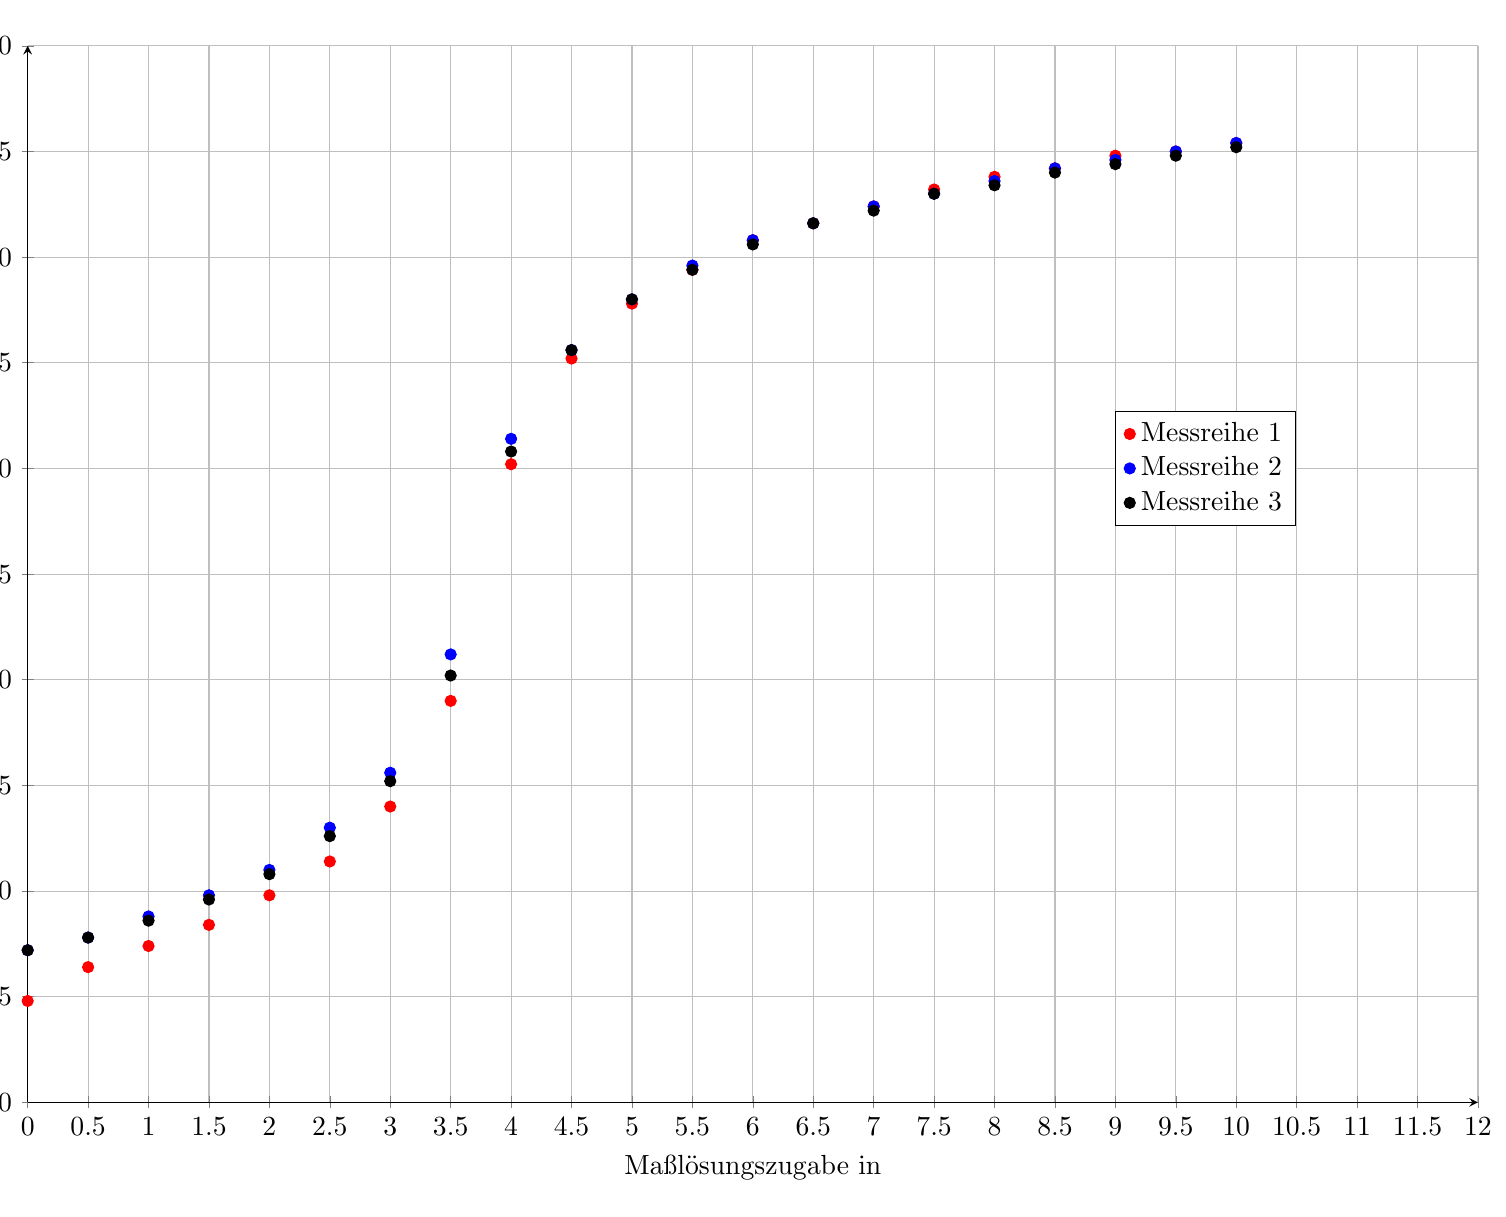
\begin{tikzpicture}[trim axis left, trim axis right]
			\begin{axis}[grid,
			axis lines = left,
			width = 20cm,
			height = 15cm,
			xmin = 0,
			xmax = 12,
			ymin = 150,
			ymax = 400,
			ytick = {150,175,...,400},
			xtick = {0,0.5,1.0,...,24},
			ylabel={Spannung in \si{\milli \volt}},
			%y label style={at={(0,0.5)}},
			xlabel={Maßlösungszugabe in \si{\milli \liter}},
			legend style={at={(0.75,0.6)},anchor=west},
			%	y dir = reverse,
			]
			\addplot [color=red, mark=*, only marks] coordinates{(0,174) (0.5,182) (1,187) (1.5,192) (2,199) (2.5,207) (3,220) (3.5,245) (4,301) (4.5,326) (5,339) (5.5,347) (6,354) (6.5,358) (7,362) (7.5,366) (8,369) (8.5,371) (9,374) (9.5,375) (10,377) };
			
			\addplot [color=blue, mark=*, only marks] coordinates{(0,186) (0.5,189) (1,194) (1.5,199) (2,205) (2.5,215) (3,228) (3.5,256) (4,307) (4.5,328) (5,340) (5.5,348) (6,354) (6.5,358) (7,362) (7.5,365) (8,368) (8.5,371) (9,373) (9.5,375) (10,377) };
			
			\addplot [color=black, mark=*, only marks] coordinates{(0,186) (0.5,189) (1,193) (1.5,198) (2,204) (2.5,213) (3,226) (3.5,251) (4,304) (4.5,328) (5,340) (5.5,347) (6,353) (6.5,358) (7,361) (7.5,365) (8,367) (8.5,370) (9,372) (9.5,374) (10,376)  };
			
			\legend{Messreihe 1, Messreihe 2, Messreihe 3}
			\end{axis}
			\end{tikzpicture}
		}
		\caption{Spannungen in Abhängigkeit der Maßlösungszugabe}
		\label{dia:potentio}
	\end{center}
\end{figure}
\FloatBarrier

\newpage

% Table generated by Excel2LaTeX from sheet 'Daten'
\begin{table}[h!]
	\renewcommand*{\arraystretch}{1.2}
	\centering
	\caption{Geradengleichungen der Messreihen 1 bis 3 für die Konduktometrie}
	\label{tab:konduk_regress}
		\resizebox{15cm}{!}{
			\begin{tabulary}{1.35\textwidth}{C|CC|CC|C}
				\hline
				&\textbf{Reaktionsgerade  (links)} & \textbf{Überschussgerade     (rechts)} & \textbf{$\boldsymbol R_1^2$}& \textbf{$\boldsymbol R_2^2$}&\textbf{Äquivalenzvolumen}\\
				\hline
				\textbf{Messreihe 1}&$\kappa_{11} =-5,186*V+544,817$ &$\kappa_{12} =13,928*V+409,343$&0,999&1,000&\SI{7,137}{\milli \liter}\\
				\textbf{Messreihe 2}&$\kappa_{21} =-5,071*V+545,483$&$\kappa_{22} =14,077*V+410,221$&0,999&1,000&\SI{7,113}{\milli \liter}\\
				\textbf{Messreihe 3}&$\kappa_{31} =-4,957*V+542,750$&$\kappa_{32} =14,129*V+407,993$&0,999&1,000&\SI{7,110}{\milli \liter}\\
				\hline
	\end{tabulary}
}
\end{table}%
\FloatBarrier

\textbf{Berechnung des Äquivalenzvolumens über Konduktometrie:}\\
Es werden die jeweiligen Regressionsgeraden gleichgesetzt und nach den Volumina umgestellt. Die Regressionsgeraden finden sich in der Tabelle \ref{tab:konduk_regress}.\\
Das Äquivalenzvolumen bezieht sich auf \SI{100}{\milli \liter} Probe.
\begin{flalign} \label{Gl:KonduAEQV}
		\kappa_{11}&= \kappa_{12}\\
		m_{11}*V_{\text{äq}}+n_{11} &= m_{12}*V_{\text{äq}}+n_{12}\\ 
		V_{\text{äq}}&= \frac{n_{12}-n_{11}}{m_{11}-m_{12}}*f_{\text{korr}}\\
		V_{\text{äq}}&= \frac{\SI{409,343}{\micro \siemens\per \centi \meter}-\SI{544,817 }{\micro \siemens\per \centi \meter}}{\SI{-5,186}{\micro \siemens\per \centi \meter\per \milli \liter}-\SI{13,928}{\micro \siemens\per \centi \meter\per \milli \liter}}*1,007\\
	&=\underline{\SI{7,137}{\milli \liter}}
\end{flalign}

\textbf{Berechnung des Äquivalenzvolumens über Potentiometrie nach \textsc{Kolthoff-Hahn}:}
Das Äquivalenzvolumen bezieht sich auf \SI{50}{\milli \liter} Probe.
\begin{flalign}\label{eq:kolthoff-hahn}
	V_{\text{äq}} &= \left(V' + \frac{\Delta V * \left(\Delta E_\text{max}-E_\text{vor}\right)}{2*\Delta E_\text{max}-\Delta E_\text{vor}+\Delta E_\text{nach}}\right)*f_\text{korr}\\[2mm]
								&= \left(\SI{3,5}{\milli \liter} + \frac{\SI{0,5}{\milli \liter}*\left(\SI{56}{\milli \volt}-\SI{25}{\milli \volt}\right)}{2*\SI{56}{\milli \volt}-\SI{25}{\milli\volt}+\SI{25}{\milli \volt}}\right)*1,007\\
								&=\underline{\SI{3,664}{\milli \liter}}
\end{flalign}

\textbf{Berechnung des Chloridgehaltes:}
\begin{flalign}
	\beta_{\ce{Cl}} &= \frac{V_{\text{äq}}*f_\text{stöch}}{V_\text{Probe}}\\[1mm]
	\beta_{\ce{Cl},1,\text{kondukt.}}&= \frac{\SI{7,137}{\milli \liter}*\SI{0,35453}{\milli \gram \per \milli \liter}}{\SI{100}{\milli \liter}}\\[1mm]
	&=\underline{\SI{25,304}{\milli \gram \per \milli \liter}}
\end{flalign}

\textbf{Berechnung des Mittelwertes:}
\begin{flalign}
\label{Gl:Mittelwert-Beispielrechnung1}
\bar{x} &= \frac{\sum_{n=1}^{N}x_n}{N}
\end{flalign}
\begin{flalign}
\label{Gl:Mittelwert-Beispielrechnung2}
\bar{x} &= \frac{\SI{25,304}{\milli \gram \per \liter}+\SI{25,219}{\milli \gram \per \liter}+\SI{25,206}{\milli \gram \per \liter}}{3}\\
&= \underline{\SI{25,243}{\milli \gram \per \liter}}
\end{flalign}
\newpage

% Table generated by Excel2LaTeX from sheet 'Daten'
\begin{table}[h!]
	\renewcommand*{\arraystretch}{1.2}
	\centering
	\caption{Zusammengefasste Äquivalenzvolumina und Chloridgehalte der Konduktometrie und der Potentiometrie}
	\label{tab:zusammen}
		%\resizebox{10.5cm}{!}{
			\begin{tabulary}{1.0\textwidth}{C|CC|CC}
				\hline
				&\multicolumn{2}{c}{\textbf{Konduktometrie}}&\multicolumn{2}{c}{\textbf{Potentiometrie}}\\
				\hline
				& \textbf{$V_\text{äq}$ in $\left[\si{\milli \liter}\right]$}& \textbf{$\beta_{\ce{Cl}}$ in $\left[\si{\milli \gram \per \liter}\right]$} &\textbf{$V_\text{äq}$ in $\left[\si{\milli \liter}\right]$}& \textbf{$\beta_{\ce{Cl}}$ in $\left[\si{\milli \gram \per \liter}\right]$} \\
				\hline
				\textbf{Messreihe 1}&7,137&25,304&3,664&25,979\\
				\textbf{Messreihe 2}&7,113&25,219&3,646&25,855\\
				\textbf{Messreihe 3}&7,110&25,206&3,659&25,943\\
				\hline
				\textbf{Mittelwert}&7,120&25,243&3,656&25,926\\
	\end{tabulary}
%}
\end{table}%
\FloatBarrier

\textbf{Berechnung der Standardabweichung:}
\begin{flalign}\label{Gl:Standardabweichung-Beispielrechnung}
s &= \sqrt{\frac{\sum_{n=1}^{N}(x_n-\bar{x})^2}{N-1}}
\end{flalign}
%	\begin{footnotesize}
\begin{flalign}
s &= \sqrt{\frac{(\SI{25,304}{\milli \gram \per\liter}-\SI{25,243}{\milli \gram \per \liter})^2+(\SI{25,219}{\milli \gram \per\liter}-\SI{25,243}{\milli \gram \per \liter})^2+(\SI{25,206}{\milli \gram \per \liter}-\SI{25,243}{\milli \gram \per \liter})^2}{2}}\\
&= \underline{\SI{5,335e-2}{\milli \gram \per\liter}}
\end{flalign}
%	\end{footnotesize}

\textbf{Berechnung des Vertrauensintervalls:}\\
\begin{flalign}
conf(\bar{x}) 	&= \bar{x}\pm \frac{t}{\sqrt{N}}*s				
\end{flalign}
\begin{flalign}
conf(\bar{x})	&= \SI{25,243}{\milli \gram \per \liter}\pm \frac{2,920}{\sqrt{3}}*\SI{5,335e-2}{\milli \gram \per \liter}\\
&= \underline{\SI{25,243}{\milli \gram \per \liter}\pm\SI{8,994e-2}{\milli \gram \per \liter}}
\end{flalign}

\textbf{Grenzwerttest:}
\begin{flalign}
	t_\text{emp} &= \frac{\bar{x}-x_\text{Grenz}}{s}*\sqrt{N}\\
								&=\frac{\SI{25,243}{\milli \gram \per \liter}-\SI{250}{\milli \gram \per \liter}}{\SI{5,335e-02}{\milli \gram \per \liter}}*\sqrt{3}\\
								&=\underline{\SI{-7,297e+03}{}}
\end{flalign}
\begin{flalign}
	t_\text{emp} &< -t_\text{crit}\\ \tag*{wahre Aussage}
	\SI{-7,297e+03}{} &< -2,920 
\end{flalign}
